\chapter{SSB in PostgreSQL}\label{sec:ssb-in-postgres}
\section{Ausführen des SSB in PostgreSQL}

% TODO: Wo werden daten generiert?
Es existiert ein GitHub-Repository ~\cite{nukoyokohama_ssb-postgres_2023}, das eine Anleitung und Skripte für das Ausführen des \ac{SSB} in PostgreSQL bereitstellt.
Zur Ausführung wurde ein Docker-Container mit dem Image \enquote{postgres-standard} erstellt.
Dabei wurden die Standardwerte der PostgreSQL-Konfiguration verwendet.
Anschließend wurden die \emph{.tbl}-Dateien und Skripte des Repositories in diesen Container geladen. 
Nach der Erstellung des Containers wird zunächst das Skript \emph{tables.sql} ausgeführt, um die Tabellen in der Datenbank anzulegen.
Danach können die Daten in die Tabellen importiert werden, indem das Skript \emph{load.sql} ausgeführt wird.
Abschließend kann der Benchmark durch die Ausführung des Skripts \emph{explain-analyze.sql} aus dem Repository durchgeführt werden.
Eine ausführliche Anleitung ist in \cref{sec:appendix-ssb-in-postgres} zu finden.
\newpage
\section{Ausführzeiten der Queries} % TODO: Ausführzeiten oder so
Die Ausführungszeiten der Abfragen in PostgreSQL werden verwendet, um die Geschwindigkeit der verschiedenen Ansätze in Redis zu vergleichen. Die Messwerte wurden durch die Berechnung des Medians von jeweils drei aufeinanderfolgenden Messungen ermittelt.
% TODO: Volle Versiond der Tabellen in Anhang packen
% TODO: Position fixen
\begin{table}[h]
\centering
\begin{tabular}{lcc}
\hline
Query & PostgreSQL \\ \hline
Q 1.1 & 283 ms       \\
Q 1.2 & 261 ms       \\
Q 1.3 & 261 ms       \\
Q 2.1 & 278 ms       \\
Q 2.2 & 267 ms       \\
Q 2.3 & 228 ms       \\
Q 3.1 & 317 ms       \\
Q 3.2 & 246 ms       \\
Q 3.3 & 217 ms       \\
Q 3.4 & 230 ms       \\
Q 4.1 & 335 ms       \\
Q 4.2 & 486 ms       \\
Q 4.3 & 260 ms       \\ \hline
\end{tabular}
\caption{Laufzeiten der SSB-Queries in Millisekunden in PostgreSQL.}
\label{tab:results-postgres}
\end{table}

% TODO: Position fixen
\begin{figure}[ht]  % figure position
    \centering      % center the image
    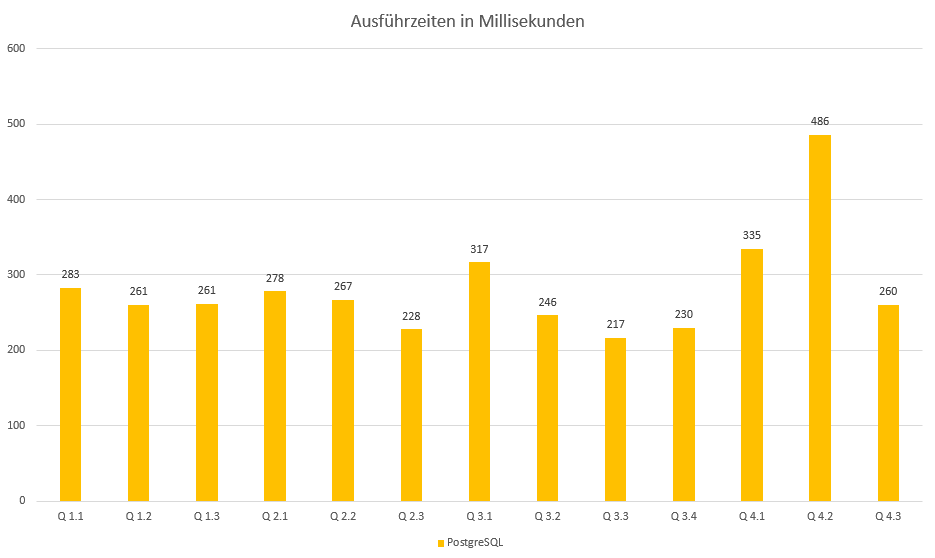
\includegraphics[width=1\textwidth]{pictures/results/results-postgres.png}
    \caption{Laufzeiten der SSB-Queries in Millisekunden in PostgreSQL.}      % caption the image
    \label{pic:results-denormalized}    % label the image for internal referencing
\end{figure}

\newpage
\section{Interpretation der Laufzeiten}
Die Laufzeiten für die verschiedenen Queries zeigen eine überraschende Konsistenz, wobei selbst komplexe Queries aus höheren Kategorien ähnlich schnell ablaufen wie einfachere aus der ersten Kategorie. Eine bemerkenswerte Ausnahme ist jedoch Query 4.2, deren Laufzeit sich deutlich von den anderen abhebt. Dies könnte entweder an der spezifischen Natur der in dieser Query verwendeten Daten liegen oder an einer weniger effektiven Optimierung durch den Query-Optimizer. In dieser Arbeit wird diese Besonderheit jedoch nicht weiter betrachtet, da das Hauptaugenmerk nicht auf einer spezifischen Untersuchung von PostgreSQL liegt und die betreffende Query nicht maßgeblich von anderen in ihrer Kategorie abweicht.
Es ist anzumerken, dass der SSB in PostgreSQL ohne extra dafür angelegte Indizes genutzt wird.